\documentclass{beamer}
\usepackage[utf8]{inputenc}

\usetheme{Madrid}
\usecolortheme{default}
\usepackage{amsmath,amssymb,amsfonts,amsthm}
\usepackage{txfonts}
\usepackage{tkz-euclide}
\usepackage{listings}
\usepackage{adjustbox}
\usepackage{array}
\usepackage{tabularx}
\usepackage{gvv}
\usepackage{lmodern}
\usepackage{circuitikz}
\usepackage{tikz}
\usepackage{graphicx}

\setbeamertemplate{page number in head/foot}[totalframenumber]

\usepackage{tcolorbox}
\tcbuselibrary{minted,breakable,xparse,skins}



\definecolor{bg}{gray}{0.95}
\DeclareTCBListing{mintedbox}{O{}m!O{}}{%
  breakable=true,
  listing engine=minted,
  listing only,
  minted language=#2,
  minted style=default,
  minted options={%
    linenos,
    gobble=0,
    breaklines=true,
    breakafter=,,
    fontsize=\small,
    numbersep=8pt,
    #1},
  boxsep=0pt,
  left skip=0pt,
  right skip=0pt,
  left=25pt,
  right=0pt,
  top=3pt,
  bottom=3pt,
  arc=5pt,
  leftrule=0pt,
  rightrule=0pt,
  bottomrule=2pt,
  toprule=2pt,
  colback=bg,
  colframe=orange!70,
  enhanced,
  overlay={%
    \begin{tcbclipinterior}
    \fill[orange!20!white] (frame.south west) rectangle ([xshift=20pt]frame.north west);
    \end{tcbclipinterior}},
  #3,
}
\lstset{
    language=C,
    basicstyle=\ttfamily\small,
    keywordstyle=\color{blue},
    stringstyle=\color{orange},
    commentstyle=\color{green!60!black},
    numbers=left,
    numberstyle=\tiny\color{gray},
    breaklines=true,
    showstringspaces=false,
}


\title{4.13.18}
\date{September 13, 2025}
\author{Bhargav - EE25BTECH11013}

\begin{document}

\frame{\titlepage}

\begin{frame}{Question}
The line $L$ is given by $\frac{x}{5} + \frac{y}{b} = 1$
passes through the point $(13,32)$. \\
The line $K$ is parallel to $L$ and has the equation
$\frac{x}{c} + \frac{y}{3} = 1.$
Find the distance between $L$ and $K$.
\end{frame}

\begin{frame}{Equation of Line $L$}
General form:
\begin{align}
\vec{n}^T \vec{x} = 1
\end{align}

For line $L$:
\begin{align}
\myvec{\frac{1}{5} & \frac{1}{b}}\myvec{x \\ y} &= 1
\end{align}

Since it passes through $\myvec{13 \\ 32}$
\begin{align}
\frac{13}{5} + \frac{32}{b} = 1 \implies b = -20.
\end{align}
\end{frame}

\begin{frame}{Equation of Line $K$}
Equation of line $K$:
\begin{align}
\myvec{\frac{1}{c} & \frac{1}{3}}\myvec{x \\ y} = 1
\end{align}

Since $K \parallel L$:
\begin{align}
\myvec{\frac{1}{c} \\ \frac{1}{3}} = \lambda \myvec{\frac{1}{5} \\ -\frac{1}{20}}
\end{align}

Thus,
\begin{align}
\lambda = -\frac{20}{3}, \quad c = -\frac{3}{4}.
\end{align}
\end{frame}

\begin{frame}{Normal Vector}
The normal vector is:
\begin{align}
\vec{n} = \myvec{4 \\ -1}
\end{align}


Distance between parallel lines:
\begin{align}
\text{Distance} = \frac{\abs{c_1 - c_2}}{\norm{\vec{n}}}
\end{align}
\end{frame}

\begin{frame}{Distance Calculation}
Substituting values:
\begin{align}
\text{Distance} &= \frac{\abs{20 - (-3)}}{\sqrt{4^2 + (-1)^2}} \\
&= \frac{23}{\sqrt{17}}.
\end{align}


Therefore, the distance between the two parallel lines is:
\begin{align}
\frac{23}{\sqrt{17}}
\end{align}
\end{frame}

\begin{frame}{Figure}
\begin{figure}[h!]
    \centering
    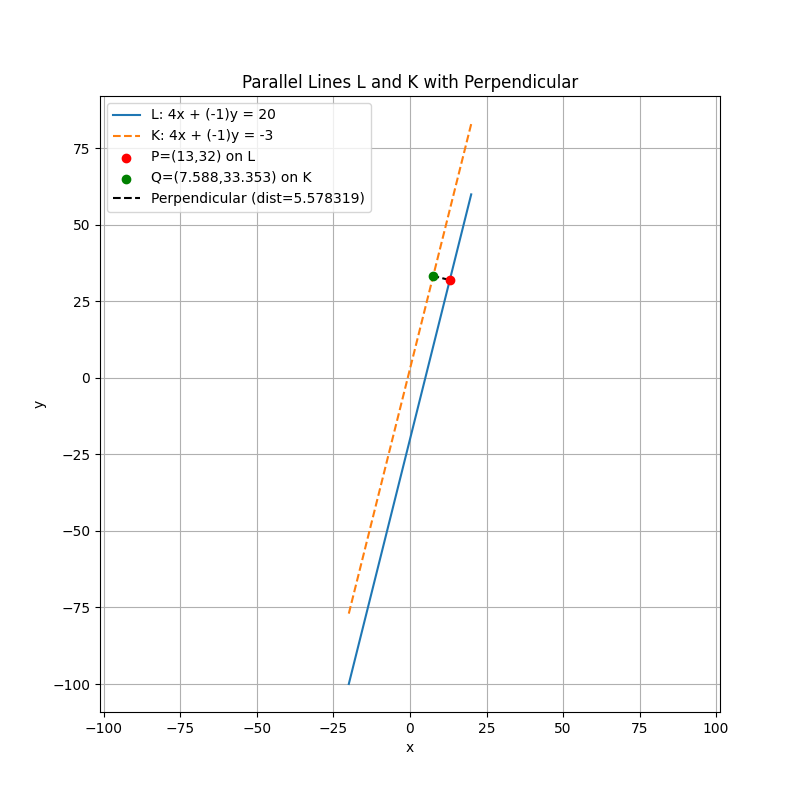
\includegraphics[height=0.5\textheight, keepaspectratio]{figs/Figure_1.png}
\end{figure}
\end{frame}

\begin{frame}[fragile]
    \frametitle{C Code}
    \begin{lstlisting}
#include <stdio.h>
#include <math.h>

double distance_between_lines(double c1, double c2, double nx, double ny) {
    double denom = sqrt(nx * nx + ny * ny);
    return fabs(c1 - c2) / denom;
}

void projection_on_line(double px, double py, double nx, double ny, double c,
                        double* qx, double* qy) {
    double denom = nx * nx + ny * ny;
    double t = (c - (nx * px + ny * py)) / denom;
    *qx = px + nx * t;
    *qy = py + ny * t;
}




    \end{lstlisting}
\end{frame}

\begin{frame}[fragile]
    \frametitle{Python + C Code}
    \begin{lstlisting}
import numpy as np
import matplotlib.pyplot as plt
import ctypes
lib = ctypes.CDLL("./liblines.so")
lib.distance_between_lines.argtypes = [
    ctypes.c_double, ctypes.c_double, ctypes.c_double, ctypes.c_double
]
lib.distance_between_lines.restype = ctypes.c_double
lib.projection_on_line.argtypes = [
    ctypes.c_double, ctypes.c_double, ctypes.c_double, ctypes.c_double, ctypes.c_double,
    ctypes.POINTER(ctypes.c_double), ctypes.POINTER(ctypes.c_double),
]
lib.projection_on_line.restype = None



    \end{lstlisting}
\end{frame}


\begin{frame}[fragile]
    \frametitle{Python + C Code}
    \begin{lstlisting}
dist = lib.distance_between_lines(c1, c2, nx, ny)
print(f"Distance between L and K = {dist:.6f}")

qx, qy = ctypes.c_double(), ctypes.c_double()
lib.projection_on_line(px, py, nx, ny, c2, ctypes.byref(qx), ctypes.byref(qy))
Q = (qx.value, qy.value)
print(f"Foot of perpendicular Q on K = {Q}")

x_vals = np.linspace(-20, 20, 400)
y_L = (nx * x_vals - c1) / ny   # line L: 4x - y = 20
y_K = (nx * x_vals - c2) / ny   # line K: 4x - y = -3

plt.figure(figsize=(8, 8))
plt.plot(x_vals, y_L, label="Line L: 4x - y = 20")
plt.plot(x_vals, y_K, "--", label="Line K: 4x - y = -3")



    \end{lstlisting}
\end{frame}


\begin{frame}[fragile]
    \frametitle{Python + C Code}
    \begin{lstlisting}
plt.scatter(px, py, color="red", zorder=5, label=f"P=({int(px)},{int(py)}) on L")
plt.scatter(*Q, color="green", zorder=5, label=f"Q=({Q[0]:.2f},{Q[1]:.2f}) on K")
plt.plot([px, Q[0]], [py, Q[1]], "k--", linewidth=1.5,
         label=f"Perpendicular (dist={dist:.3f})")
plt.xlabel("x")
plt.ylabel("y")
plt.title("Parallel Lines L and K with Perpendicular")
plt.legend()
plt.grid(True)
plt.axis("equal")
plt.savefig("/Users/bhargavkrish/Desktop/BackupMatrix/ee25btech11013/matgeo/4.13.18/figs/Figure_1.png")
plt.show()

    \end{lstlisting}
\end{frame}

\begin{frame}[fragile]
    \frametitle{Python Code}
    \begin{lstlisting}
import numpy as np
import matplotlib.pyplot as plt

def distance_between_lines(c1, c2, nx, ny):
    return abs(c1 - c2) / np.hypot(nx, ny)

def projection_on_line(px, py, nx, ny, c):
    denom = nx*nx + ny*ny
    t = (c - (nx*px + ny*py)) / denom
    qx = px + nx*t
    qy = py + ny*t
    return qx, qy

px, py = 13.0, 32.0   
a = 5.0              
b = py / (1 - px / a)



    \end{lstlisting}
\end{frame}

\begin{frame}[fragile]
    \frametitle{Python Code}
    \begin{lstlisting}
print("Computed b:", b) 
nL = np.array([1.0/a, 1.0/b])
scale = 20.0
nx, ny = (nL * scale).tolist()   
c1 = 1.0 * scale              
c2 = -3.0
dist = distance_between_lines(c1, c2, nx, ny)
qx, qy = projection_on_line(px, py, nx, ny, c2)
print("Distance between L and K:", dist)
print("Foot Q on K:", (qx, qy))
x_vals = np.linspace(-20, 20, 400)
# CORRECT formula: y = (c - nx*x) / ny
y_L = (c1 - nx * x_vals) / ny
y_K = (c2 - nx * x_vals) / ny
plt.figure(figsize=(8, 8))

    \end{lstlisting}
\end{frame}

\begin{frame}[fragile]
    \frametitle{Python Code}
    \begin{lstlisting}
plt.plot(x_vals, y_L, label=f"L: {int(nx)}x + ({int(ny)})y = {int(c1)}")
plt.plot(x_vals, y_K, "--", label=f"K: {int(nx)}x + ({int(ny)})y = {int(c2)}")
plt.scatter(px, py, color="red", zorder=5, label=f"P=({int(px)},{int(py)}) on L")
plt.scatter(qx, qy, color="green", zorder=5, label=f"Q=({qx:.3f},{qy:.3f}) on K")
plt.plot([px, qx], [py, qy], "k--", linewidth=1.5, label=f"Perpendicular (dist={dist:.6f})")
plt.xlabel("x"); plt.ylabel("y")
plt.title("Parallel Lines L and K with Perpendicular")
plt.axis("equal")
plt.grid(True); plt.legend()
plt.savefig('/Users/bhargavkrish/Desktop/BackupMatrix/ee25btech11013/matgeo/4.13.18/figs/Figure_1.png')
plt.show()

    \end{lstlisting}
\end{frame}

\end{document}
